\section{Infrastructure}
\subsection{Domain information}

Here we work our way piece by piece {\bf from rough to detailed} information.
Therefore we first have to get a technical overview of the company. Since we
usually already know the name of the company or even the domain name, this
information is generally sufficient to determine how the company is
structured.
\begin{figure}
  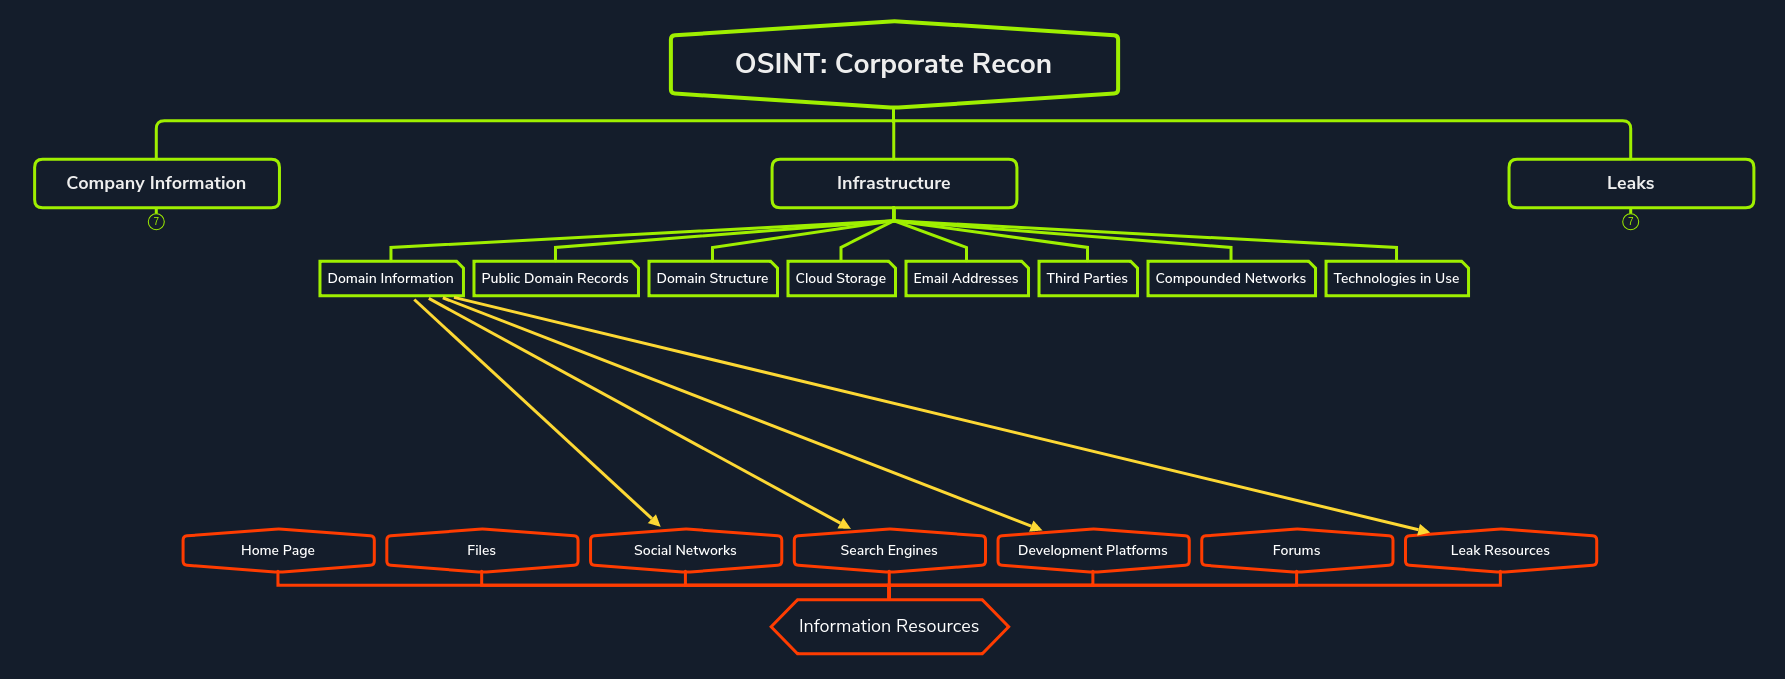
\includegraphics[width=\linewidth]{recon/osint/images/infra-domain-info.png}
  \caption{OSINT Domain information}
  \label{fig:osint-domain-info}
\end{figure}

The element we focus on in the first phase of the company's infrastructure
investigation is the domain names we can find. We then go into each domain and
get an overview of the subordinate structure that contains 
\begin{itemize}
        \item Netblocks
        \item Name Servers
        \item Mail Servers
        \item subdomains
        \item hosts/IP addresses.
\end{itemize}

We can classify the rough structure into three categories:
\begin{itemize}
        \item Public Records:  	
        \item Third Parties 	
        \item Domains
\end{itemize}

\subsubsection{Social Networks}
We often find references to domains or subdomains on social media platforms.


\subsubsection{Search Engines}
One of the most efficient methods of searching for domains is offered by
various search engines. In this case, we cannot focus on a domain name, but we
have to work with general company terms, such as the company name, the name of
the application or service, and others.

Another excellent way to find out information about our target domain is to use
a particular Search Engine Optimization (SEO) field called backlinks. 

One of such backlinks analyzers is
\href{https://app.neilpatel.com/en/seo_analyzer/backlinks}{Ubersuggest}.

\subsubsection{Development Platforms}
Development platforms also offer excellent information resources for us here,
as we will often find code that sometimes even provide information that is
dangerous for the company. This information can range from IP addresses and
hostnames, configuration files to credentials.

\subsubsection{Leak Resources}
Once we have a list of the company's domains, we can use it to look for known
anomalies that affect the company and the corresponding domain. One of the best
sources of information for this is
\href{https://www.virustotal.com/}{VirusTotal}, where we can scan each domain
for suspicious activity.


Another source that searches against many different developer platforms is
\href{https://searchcode.com/}{Searchcode}. It searches all possible codes for
terms that we specify in the search and shows us the sources accordingly.

\subsection{Public Domain Records}

Public domain records offer us excellent opportunities to trace the company's
information technology infrastructure structure. With the right arrangement and
knowledge of what the records are for and what information they contain, they
can provide us with information about the company's Internet presence. To get
this, we need to find out at least four components:
\begin{verbatim}
1. Netblocks / CIDR 	2. ASN 	3. DNS Servers 	4. Mail Servers
\end{verbatim}

This gives us an overview of which systems are accessible from the internet, in
which address range they are located, which IP neighbors they have, and how the
interaction between them takes place.

\begin{figure}
  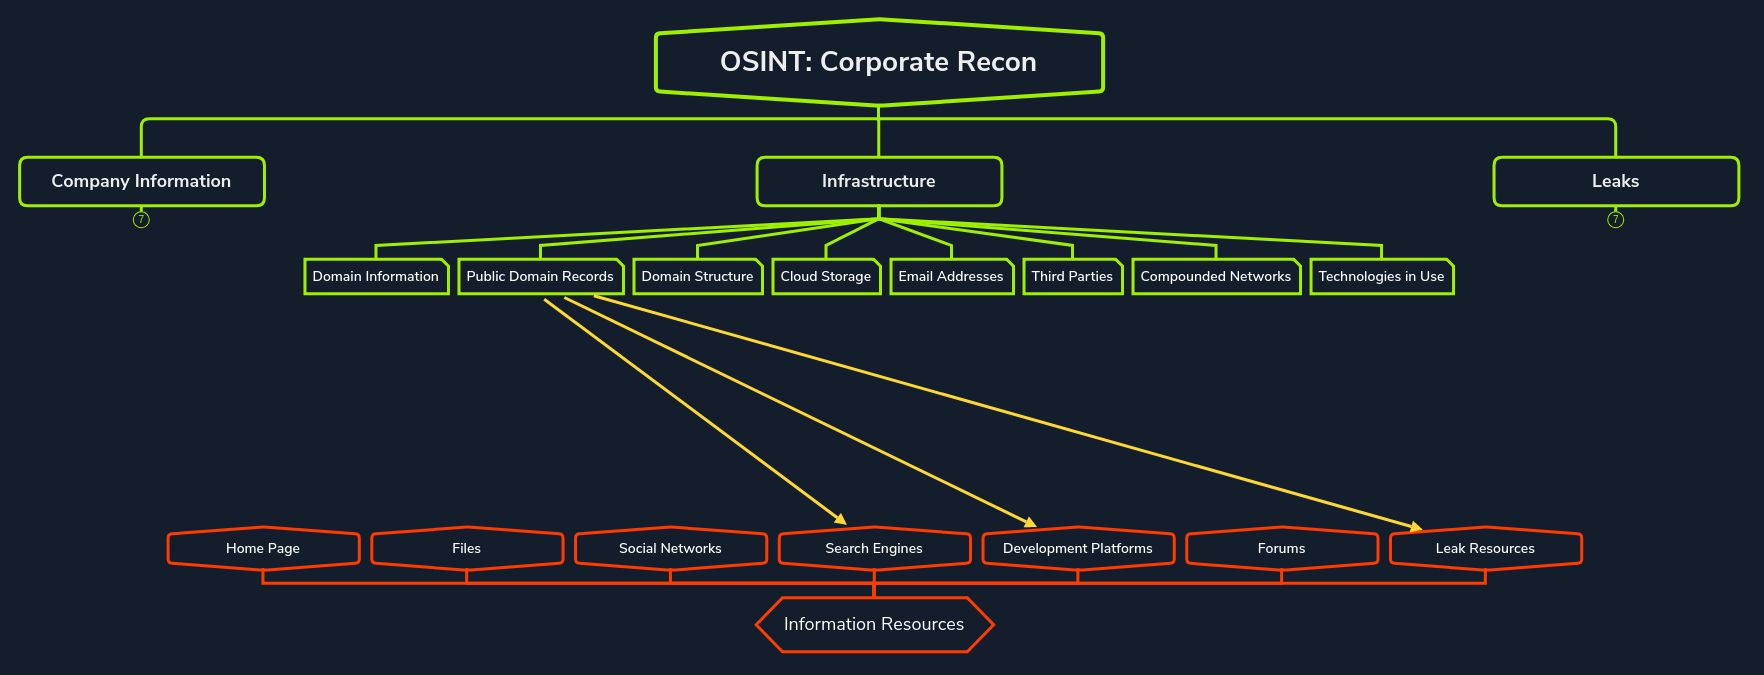
\includegraphics[width=\linewidth]{recon/osint/images/infra-pub-records.png}
  \caption{OSINT Domain public records}
  \label{fig:osint-infra-pub-records}
\end{figure}

\subsubsection{Search Engines}
The minimum information we need to get from our client, apart from the company's
name, is a domain or at least an IP address to start with. The scope of this
can vary greatly.

{\bf 1. Netblocks / CIDR}

During a black-box penetration test, our client will often only provide the
domain name. We can use this to find out a lot of helpful information. First of
all, we should find the IP address of the main webserver(s) and the IP address
range(s) / CIDR. For this, we can use the following command.
\begin{verbatim}
host www.inlanefreight.com
\end{verbatim}
Now that we have the IP address of the web server, we can find out which IP
address range it is located in. By default, we can work with the Whois protocol
used by a distributed database system to retrieve information about internet
domains and IP addresses and their owners.
\begin{verbatim}
whois 134.209.24.248
\end{verbatim}
We can also search the WHOIS databases for the company name. We are often given different identification numbers (mnt-ref), which we can use for further searches. These stand for the maintainer objects, which are used as a reference for the organization objects.
\begin{verbatim}
whois -B --sources RIPE,ARIN target-company
\end{verbatim}
We can also query the individual databases and identify the associated netblocks.
\begin{verbatim}
whois -h whois.arin.net target-company | grep -v "#" | sed -r '/^\s*$/d'
\end{verbatim}
Here is the \href{https://www.arin.net/resources/registry/whois/rws/cli/}{ARIN
list} of other flags we can use to get more information from
the maintainer objects. 


{\bf 2. ASN}

We can also see another crucial piece of information here, the {\bf OrigisAS}.
This is the {\bf Autonomous System Number (ASN)}. This number is unique and is
made publicly available so routing information can be exchanged with other
systems. This is done with specific IP prefixes, which we can use to find out
the netblocks ({\bf public ASNs}). There are also {\bf private ASNs} intended
for systems that only communicate via a provider. Other protocols such as the
{\bf Border Gateway Protocol (BGP)} are used if this is the case. We can use
\href{https://mxtoolbox.com/SuperTool.aspx}{MXToolbox} and its {\bf ASN Lookup}
option with the ASN to find out how many subnets the owner has.

Another way to get more information about the domain is to use the
\href{https://lookup.icann.org/lookup}{ICANN lookup}. Each domain is registered
to an organization or person with a unique ID, which provides information about
when the domain was created and expires.

{\bf 3. DNS Servers}

DNS servers are essential services today because they help the regular user
reach the web services they want.  It is often the case that companies own
several domains, and accordingly, these domains can offer different attack
vectors that can affect each other. The next step is to look at the DNS records
of our target domain using dig. Dig is a DNS lookup utility that can be used to
obtain publicly available information from DNS.

\begin{verbatim}
dig any inlanefreight.com
\end{verbatim}

If we now take a closer look at the records, we see that the SOA record shows
another domain, infreight.com. Therefore we will also look at these if the
scope allows us to do so. In this case, we assume that we have permission to
test this domain as well.

Another source we can use, which gives us a much better representation of the
DNS servers' records, is \url{https://dnsdumpster.com/}{DNSdumpster}.

Here we can see the entries for the respective DNS servers and the locations of
the corresponding hosts and servers. Then we see the respective IP addresses
and corresponding subdomains that could be obtained from the entries.
Additionally, DNSdumpster can sometimes show us the services running on the
server if it can passively identify them. Finally, at the bottom of the page,
we can see a domain map that shows the relationships between the servers
connected with the records.

{\bf 4. Mail Servers}

Mail Server / Exchange server ({\bf MX}) is one of the most critical services
today, as it ensures that our emails reach the desired communication partners.
Other servers use it as an interstation (relay) for sending spam or viruses. It
often happens that MX servers do not only use specially registered servers as
relays. This gives us the possibility to perform an {\bf Open Relay Attack}.

MX servers represent a massive attack vector. There is nothing worse for a
company apart from a complete compromise than the fact that all unencrypted
emails can be intercepted and read. This means that not only GDPR guidelines
have been violated by requiring the company to ensure that customer data is
kept confidential, but it also significantly impacts customer satisfaction and
customer trust, which will be significantly damaged.

\href{https://mxtoolbox.com/}{MXtoolbox} offers an excellent service to test
the MX servers for Open Relay.


\subsubsection{Development Platforms}

Searching for code on developer platforms can bring surprising results. Apart
from already highly sensitive data such as user names and passwords, we can
also find {\bf configuration files} containing the latest administration settings. We
can use \href{https://searchcode.com/}{searchcode} again with specific strings
and known {\bf IP addresses} or {\bf domain names} to get such results.
However, in this case, we need a basic understanding of the configuration
files, how they can look, and which variables can be used for DNS
configuration.

\subsubsection{Domain structure}
Now that we have gathered a lot of information, we need to focus on the
intelligence of this process and create an {\bf overview of the domain}, and
analyze our results. We should take our time because the better we understand
the structure of the domain, the easier it will be to take the appropriate
steps later. Furthermore, we narrow down the goals and seek out the {\bf low
hanging fruit} of all the systems that promise the best possible results for us.


\begin{figure}
  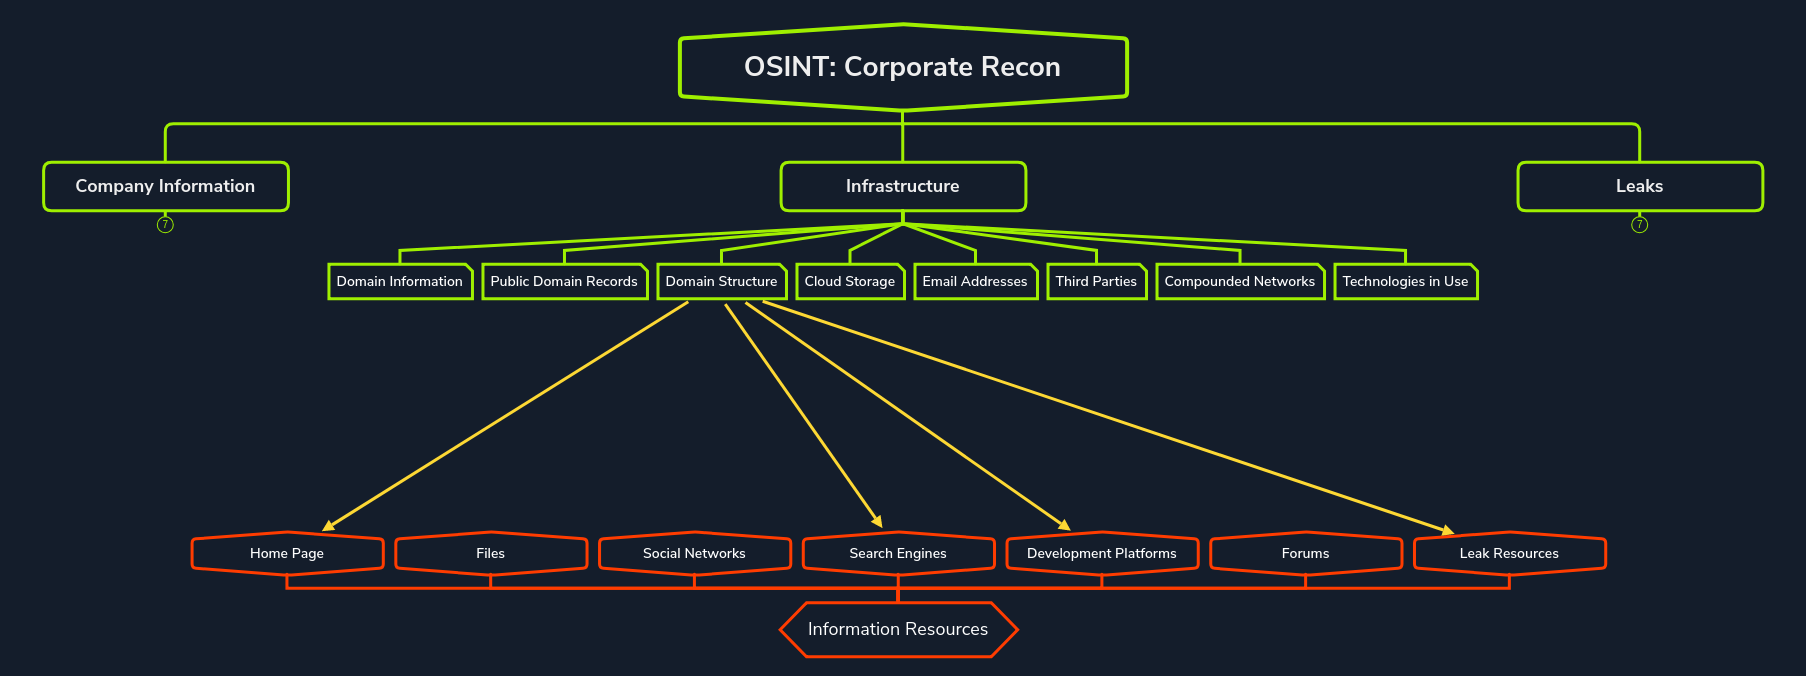
\includegraphics[width=\linewidth]{recon/osint/images/infra-domain-structure.png}
  \caption{OSINT Domain structures}
  \label{fig:osint-infra-domain-structure}
\end{figure}
This preparation can take several hours of study but save us time in the
following steps because we will not test each system blindly, but proceed
methodically, organized and structured. This represents the professionalism of
our work and gives a much better impression in the reports for our customers.

\subsubsection{Home Page}
Countless websites link to other subdomains. Therefore, we should always pay
attention to each clickable area on every web page owned by the company.

\subsubsection{Search Engines}

Since we are still in the passive information gathering phase, we should use
passive techniques to find out more subdomains. For this, we can use a tool
called \href{https://github.com/UnaPibaGeek/ctfr}{CTFR}. It uses Certificate
Transparency logs from
\href{https://www.certificate-transparency.org/}{Certificate Transparency} and
\href{https://crt.sh/}{crt.sh}.

\begin{verbatim}
./ctfr.py -d inlanefreight.com | grep -v "[-]"
\end{verbatim}

We can now use CTFR for each subdomain in a For-Loop because there may be other
subdomains in the respective subdomains. After we have collected and documented
all passive results, we can use a simple For-Loop in Bash to determine the
corresponding IP address for each subdomain.

Then we can use \verb+whois+ and \verb+ipcalc+ to find out the IP ranges for
the respective IPv4 addresses.


There are many different resources we can use to find out the IP addresses of
our target company. One of the best and most used resources is
\href{https://www.shodan.io/}{Shodan}. Shodan also offers a
\href{https://cli.shodan.io/}{CLI version} that we can install. This allows us
to query, filter, and save the results directly from the command line, making
documentation much more manageable.

\begin{verbatim}
shodan domain <TARGET-DOMAIN> |
    grep -w "A" | cut -d"A" -f2 | cut -d" " -f7 | sort -u > IPv4s.txt

for ip in $(cat IPv4s.txt);do shodan host $ip;done
\end{verbatim}

After this, we can use \href{https://ipinfo.io/}{IPinfo.io}. This resource
provides an excellent way to 
identify the subnets and hosting providers. Furthermore, we can use Spyse to
search for additional subdomains by entering the top and second-level domains
(e.g., target-company.htb).

Another great way to quickly search for subdomains is
\href{https://subdomainfinder.c99.nl/index.php}{C99.nl}. We should remember
that we should always use multiple sources to find all subdomains if possible.
This is because we will rarely have situations where a single source provides
us with all available subdomains.


With the IP addresses and subdomains, we can determine how many and which
subdomains are {\bf virtual hosts}. Some good sources that we can use are
\href{https://pentest-tools.com/information-gathering/find-virtual-hosts}{Pentester-Tools}
and \href{https://hackertarget.com/}{Hacker-Target}.
With the IP addresses and subdomains, we can determine how many and which
subdomains are virtual hosts (vHosts). Some good sources that we can use are
Pentester-Tools and Hacker-Target.

\subsubsection{Development Platforms}
or the developer platforms, we should be on the lookout for all possible files,
as eventually, any of them may contain hints about domain names or IP
addresses. Configuration files are of particular interest, as they may contain
access data and have fixed IP addresses and (sub)domains. For this, we can
again use \href{https://searchcode.com/}{Searchcode} to find files of this kind
quickly.

Another very interesting source of information is the
\href{https://www.seoptimer.com/}{SEOptimer}. This is an SEO analysis tool that
examines and evaluates the entire website for individual components.In general,
marketing tools are designed to evaluate visitors' interactions on the website
and allow SEO specialists and web designers to make the appropriate adjustments
to improve the rating or create a better UX. Since they work a lot with links,
we will likely find out a lot of helpful information.

\subsubsection{Leak Resources}

Leak resources are unauthorized publications of information. This term is broad
and can therefore include many different information components. These
resources also include databases with datasets containing information about our
target company. At the end of 2017, Rapid7 started
\href{https://opendata.rapid7.com/sonar.fdns_v2/}{Project Sonar}, which
collects and stores responses forwarding DNS requests. DNS records such as A,
AAAA, CNAME, and TXT lookups are stored at certain intervals in individual GZIP
files in the form of JSON. These databases are extensive and can exceed 30GB in
compressed format. They contain (sub)domains, record types, and the
corresponding IP addresses. This information resource serves as an updated and
valuable resource for us to understand our target company's domain better.

\subsection{Cloud storage}

\begin{figure}
  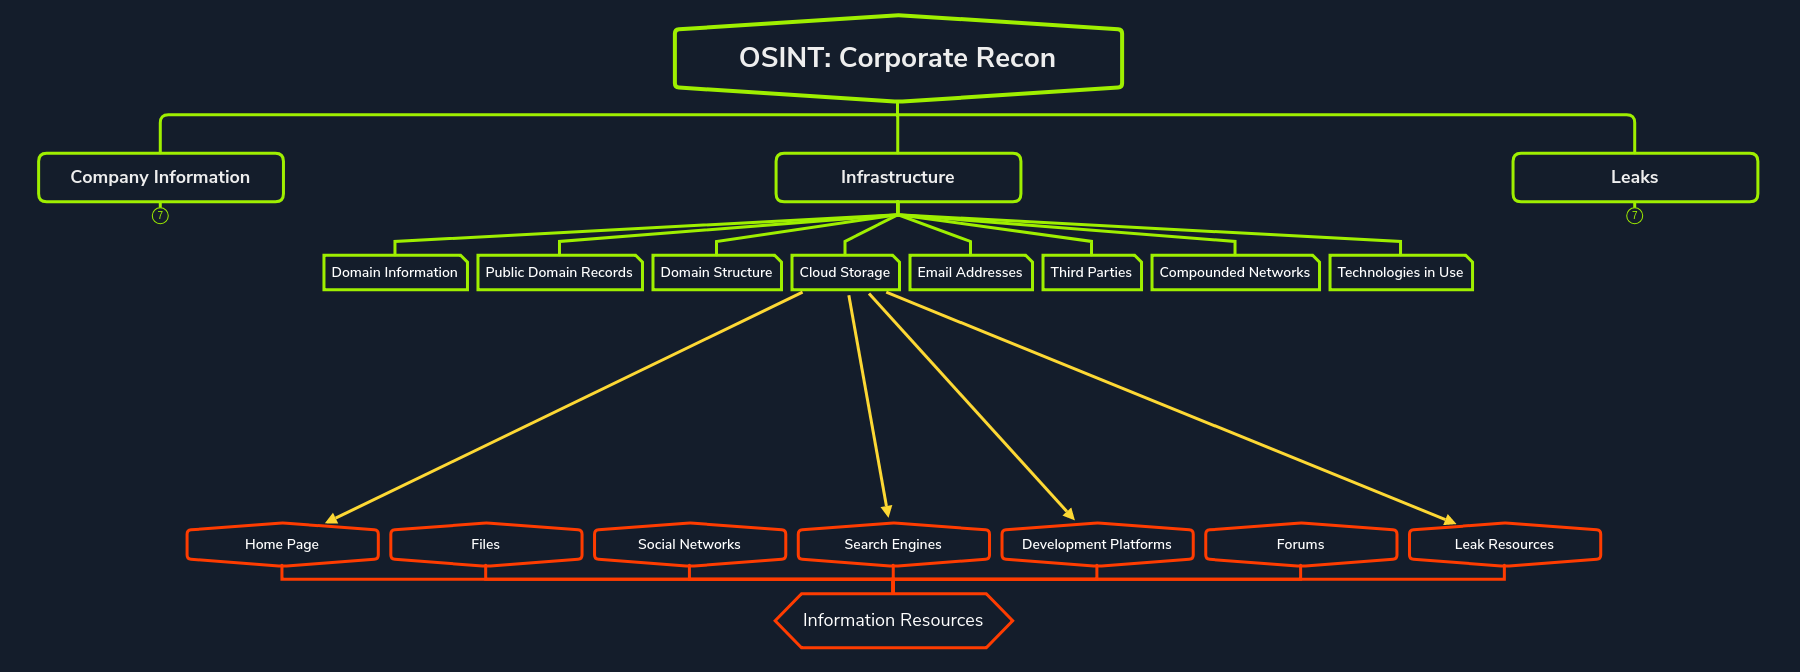
\includegraphics[width=\linewidth]{recon/osint/images/infra-cloud.png}
  \caption{OSINT Infra cloud}
  \label{fig:osint-infra-cloud}
\end{figure}

We can now resolve the domains found into IP addresses and compare them to the
netblocks for these three cloud providers. If we find any IP addresses within
these IP ranges, we can assume that it is a cloud provider. For us, the most
critical component in the corporate use of a cloud provider is open cloud
storage because if they have been misconfigured, they are publicly accessible
and viewable. Some of those cloud providers are, but not limited to:
\begin{verbatim}
 				
Cloud Provider 	    GCP 	                Azure 	    AWS 	    DigitalOcean
Open Cloud Storage 	Google Storage Bucket 	Block Blob 	S3 Buckets 	Spaces
\end{verbatim}

We can also automate this process with the tool
\href{https://github.com/oldrho/ip2provider}{ip2provider.py}. This will
automatically compare the IP addresses with the netblocks and show if they are
successful matches.

\begin{verbatim}
cat Target_Company.IPv4s | ./ip2provider.py
\end{verbatim}

\subsubsection{Home Page}
When searching for cloud buckets, one factor makes it difficult for us to
identify the bucket belonging to the company. This is that everyone can create
their own name for the desired bucket. This means that anyone can create a
bucket with the target company's name without it belonging to the company.

Here we can also find a list of URLs from which we can see which cloud provider
the storage belongs to and where we could find it.

\begin{verbatim}
Cloud Provider 	URL
GCP 	https://www.googleapis.com/storage/v1/b/<bucket-name>/iam

Azure 	https://<bucket-name>.core.windows.net/<container>/
	i   https://<bucket-name>.blob.core.windows.net/<container>/

AWS 	https://<bucket-name>.s3.amazonaws.com
	    https://s3-<region>.amazonaws.com/<company-name>
\end{verbatim}

Almost all (~95\%) vulnerabilities in the cloud happen due to misconfigurations. These misconfigurations include, but are not limited to:
\begin{itemize}
    \item   ACLs
    \item   Bucket Policies
    \item   Service Control Policies
    \item   Public Access Blocks
    \item   IAM Policies
\end{itemize}

Cloud environments extend the penetration testing process enormously. However,
this does not affect the OSINT process since we ultimately use public resources
to not interact with our target company. Further investigation of cloud buckets
will be covered in another Module, as we need to investigate and understand the
setup and the individual configuration options to work with them effectively.
However, we already know enough to find open cloud buckets. Whether they are
open and whether we can see the content on them requires interaction.
Therefore, we will stop after finding them, and in the next stage, we will deal
with them and enumerate them.


The first information resource often used for this purpose is the company's
website. Buckets are often used as a source for the web servers and their
contents are linked accordingly.

We can also use this content and the names of the files or the company's full
domain name (i.e., www-target-company-com) for Searchcode to see if they are
publicly retrievable and if there might even be more information resources for
them. To do this, we take the name of the file and can, for example, look for
other cloud providers to see if they are available there. The more unique the
name of the file is, the more accurate the results will be. These are then
easier to identify and connect to the target company.

\subsubsection{Search Engines}
If files have been tagged or named in conjunction with the company name, we can
use the search engines we know and filter the results based on the cloud
providers. Aside from file names and company names, we may also use employee
names or application names if they appear unique. For this, we can set the
known domains from the cloud providers as the assumed content (with the
\verb+inurl:+ tag) for our results. This will reduce the results only to those
that contain this domain. Finally, we know that the buckets' label will not
necessarily have the name or label we have already seen. For this, search
engines help us to expand our search scope but also to reduce it.

Another information resource that serves very well for finding such buckets is
the \href{https://buckets.grayhatwarfare.com/}{GrayHatWarfare Project}. This
project is an online tool that searches for open cloud buckets and archives
them. This is one of the most widely used tools currently, and it also gives
excellent results since it contains an enormous amount of records.

The GrayHatWarfare Project offers us many different options, such as filtering
by buckets, files, file types, keywords, and even an API interface. We can
search these buckets for files and see which of them might be relevant for us.
The advantage is that we do not have any interaction with buckets owned by the
target company as long as we do not explicitly call the files or list them via
the CLI.

\subsubsection{Development Platforms}

Again, developer platforms are of great use to us, as we can search code to
find out if specific files exist in connection with the cloud buckets. As we
know, {\bf Searchcode} also redirects us to the resource that points to the
corresponding file. Often used strings in these files are {\bf AccountName} and
{\bf AccountKey}, used for authorization (like username and password).

These files usually contain the {\bf IP addresses} or the {\bf bucket names} for the
corresponding cloud storage. We can use these to search again on {\bf
GrayHatWarfare}
and filter out the results. Therefore, if we follow these files and examine
them more closely, we will most likely find a lot more helpful information that
we will need for our documentation and further research. 

\subsubsection{Leak Resources}

Another source that can point us to the buckets and forward them is the
aforementioned \href{https://opendata.rapid7.com/sonar.fdns_v2/}{Rapid7
database}. Since this works with the forward DNS requests and responses and
documents those, it is even very likely that we will find entries that will
show us the corresponding buckets.


\subsection{Email Addresses}
Identifying existing email addresses can also provide us with a massive attack
vector that we can use to our advantage. We can use emails in many ways. Among
other things, email can be used not only for phishing attacks, but we can also
analyze the traffic of these to identify which is the "central" point for the
processing of emails. After all, this will have by far the most sent emails. We
can also subscribe to newsletters and analyze their headers with MXTools, which
will also show us the route of the email and its security settings.

\begin{figure}
  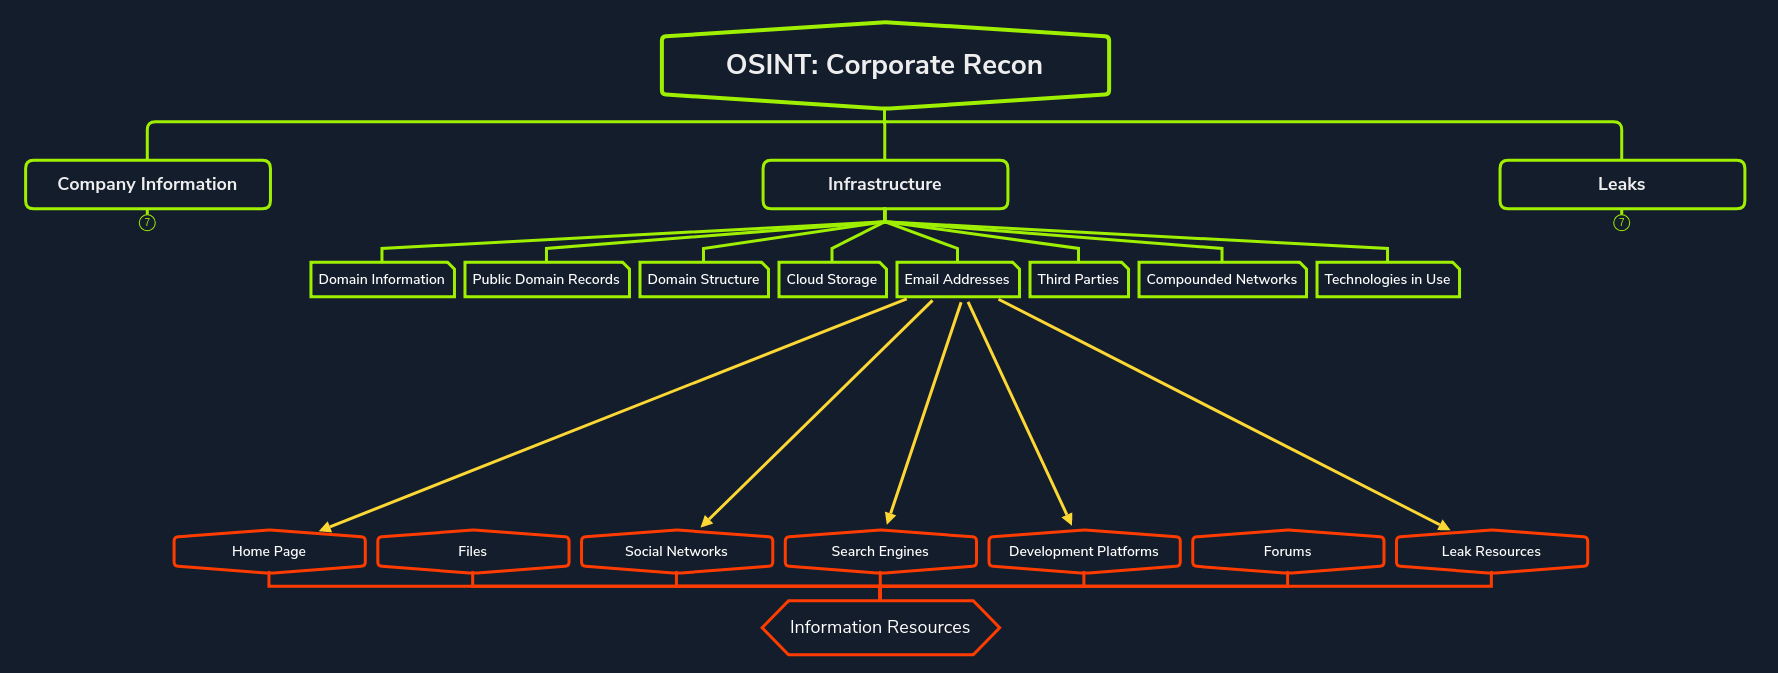
\includegraphics[width=\linewidth]{recon/osint/images/infra-emails.png}
  \caption{OSINT Infra Emails}
  \label{fig:osint-infra-emails}
\end{figure}
Email addresses may have different structures even within the same company. One
of the most common examples is when the first and last name
(first.lastname@domain.tld) is used in the email address. However, the email
addresses can be created with usernames (username@domain.tld) not to show the
user's full name.

\subsubsection{Home Page}

The company's website is often the stop for us to find out interesting
information. In most cases, we find the first points of contact through email
addresses on the contact or about page. We may find email addresses for
personal contact with the individual, for business and informational purposes,
as well as for job applications or even department heads. This also helps us to
understand very well how the internal infrastructure may be set up. In larger
companies with multiple locations, the individual departments are managed with
the country codes available in the email addresses. Therefore, we can often
find information on the offices or local information pages. It is helpful if
the individual departments and their functions are described on this page,
which can help us to understand the internal infrastructure better.

Finally, companies often try to use as short terms as possible, as these are
easier to remember and require less effort to type. Therefore, the domains for
the email addresses can be different but still belong to the same domain. For
example, if we find a company with the name Target-Company.com, the abbreviated
variant could be TarCom.com or TC.com, if they are still available.


\subsubsection{Social Networks}

As we already know, many conversations occur on social networks, and therefore
a lot of information is shared. We can also find email addresses there that
point to particular addresses for exceptional cases. Here we can use the
combination of social networks and search engines to find them. In the search
engines, such as Google, we then use the corresponding Google dorks
(\verb+inurl:+ and \verb+intext:+) to optimize social networks' results.


For the dork \verb+inurl:+ we set the domain of the corresponding social
network we are looking for. Next, we use the dork \verb+intext:+ with the
extension for an email address (\verb+@domain.tld+) that belongs to our target
company. This then gives us some results that we can further investigate to
establish further links.

Another critical role for email addresses is their {\bf reputation}. This could
tell us whether the corresponding email address has already been used for spam
activities, has been blacklisted, whether {\bf SPF} or {\bf DMARC} is used, and
much more. To get this information, we can use the information resource called
\href{https://emailrep.io/}{Emailrep}. Apart from the information we get from
it, using the API is very useful for us as we can easily use it with cURL.
\begin{verbatim}
curl -s emailrep.io/info@target-company.com
\end{verbatim}

It for example provide the information if the email is {\bf spoofable}


\subsubsection{Search Engines}

Once we have worked through the most used social networks, we can use the
search engines to look for other information resources, including company email
addresses. We can use the same Google Dork (\verb+intext:+) to filter the
results and match them with the existing list.

On the first page of the 18,000 results, we can already find an email interface
of the company based on this simple usage, which can and should also be
investigated in more detail later (if the scope allows this). Suppose we
encounter a case where a large number of results appear that belong to a single
domain. In that case, we can also use the dorks to exclude specific information
resources by placing a minus in front of the dork (\verb+-inurl:+).

A very efficient tool for this is called
\href{https://github.com/laramies/theHarvester}{theHarvester}~\ref{tool:theharvester}. This tool
    searches the information resources we provide, such as Google, Netcraft,
    Spyse, Twitter, and others for entries. Some of these services offer API
    keys that are bound to the corresponding account to execute the requests.
    Often there are limits on the number of requests we can send.
\begin{verbatim}
theHarvester.py -d inlanefreight.com -b google,hunter,netcraft,spyse,twitter,dnsdumpster
\end{verbatim}


\subsubsection{Development Platforms}

Apart from insight into the company's technologies and source code, development
platforms also serve very well to find out email addresses. Developers' email
addresses are interesting, as they are often linked on different platforms,
which we can then investigate and analyze later in the staff investigation
phase. We will go into this in another Module called {\bf OSINT: Staff
Investigation}.

Here we can also use the combination of the developer platforms and the search
engines to find out the developers' email addresses. Just as we used the Google
Dorks for social networks, we use them again, only this time for the developer
platforms.

Another useful combination is searching for images in connection with the email
addresses. This search option is usually overlooked, as most people do not see
any relationship between email addresses and images. However, users often
upload images linked to such an email address in the text or in some other
way.

A small difference is that we no longer use the \verb+inurl:+ dork for the
information resource but \verb+intext:+ to extend the linking to the individual
information resources.

\subsubsection{Leak Resources}

In principle, leaks can be displayed in any form. What counts is how, where,
and what exactly was found. It becomes much more relevant when this information
is used to complete and adapt an attack against the company. Here, the attitude
of the developers to the information they discuss in public plays a significant
role. Moreover, some are unaware that the information they share can be viewed
publicly, assuming no one is looking for it. Furthermore, it is precisely this
kind of attitude that often puts companies at risk of being attacked.


Moreover, several factors come together because even if the developers are
aware of it, misconfigurations are another factor that makes even their
settings seem ineffective. Misconfigurations can even lead to calendars with
appointments being publicly visible.

Email addresses often play a significant role in this field, as they are linked
via a wide variety of platforms. Let us consider that passwords are often used
repeatedly across multiple platforms. The risk is relatively high that if we
can find a password for an email address and log it into a company's email
interface, this will lead to significant information leakage that may even
result in full compromise. One of the most effective tools that can be used to
support linking is \href{https://github.com/khast3x/h8mail}{h8mail}.

\begin{verbatim}
8mail -c h8mail_config.ini -t first.lastname@target-company.com
\end{verbatim}

From the results, we can see that the email address we analyzed is contained in
seven different databases whose passwords can be viewed. Another option is to
use the service of \href{https://haveibeenpwned.com/}{HaveIBeenPwned} to
determine if any of the email addresses we found are already in databases that
contain passwords for them and have been compromised.

HaveIBeenPwned also goes through all available databases and checks the entries
for the existence of the email address we entered. It will show us which
platforms have been affected by this data's loss if it is there.

\subsection{Third Parties}
Identifying third-party providers requires a little more manual work and
research. Since we know that there may be severe legal consequences for us,
including a criminal charge, we should look at this issue here. In the case of
a black-box penetration test, we must pay close attention to which third-party
providers offer services to our target company.

However, this does not mean that we are not allowed to test systems from
third-party suppliers. For this purpose, "Penetration Testing Authorisation
Forms" exist, which must be filled in and submitted. This is to inform the
third-party vendors that they will most likely receive alerts for the specific
systems and should be aware that this is done with our intent. This will also
prevent our Internet Service Provider (ISP) from being contacted and blocking
our access to the internet. It will also stop us from being charged for
attacking the hosts.

We should not use attacks such as DDOS unless all parties have agreed to do so
not to restrict the services we provide to other users. But here, too, there
are always precise specifications (Penetration Testing Rules of Engagement)
from third-party suppliers that we have to follow.

If no forms are available from the third-party provider, our customer must
contact the third-party provider and obtain permission. Otherwise, our customer
must fill out and submit the documents and provide us with confirmation of
permission to test the systems.

\begin{itemize}
    \item Amazon Web Services
        \url{https://aws.amazon.com/forms/penetration-testing-request}
    \item Digital Ocean
        \url{https://cloud.digitalocean.com/support/tickets/new}
    \item Google Cloud 	\url{https://support.google.com/cloud/answer/6262505?hl=en}
    \item Microsoft Azure
        \url{https://security-forms.azure.com/penetration-testing}
\end{itemize}

By now, we should have gathered enough information to keep an eye out for the
third parties. When looking for them, we must assemble an extensive collection
of information resources.

\begin{figure}
  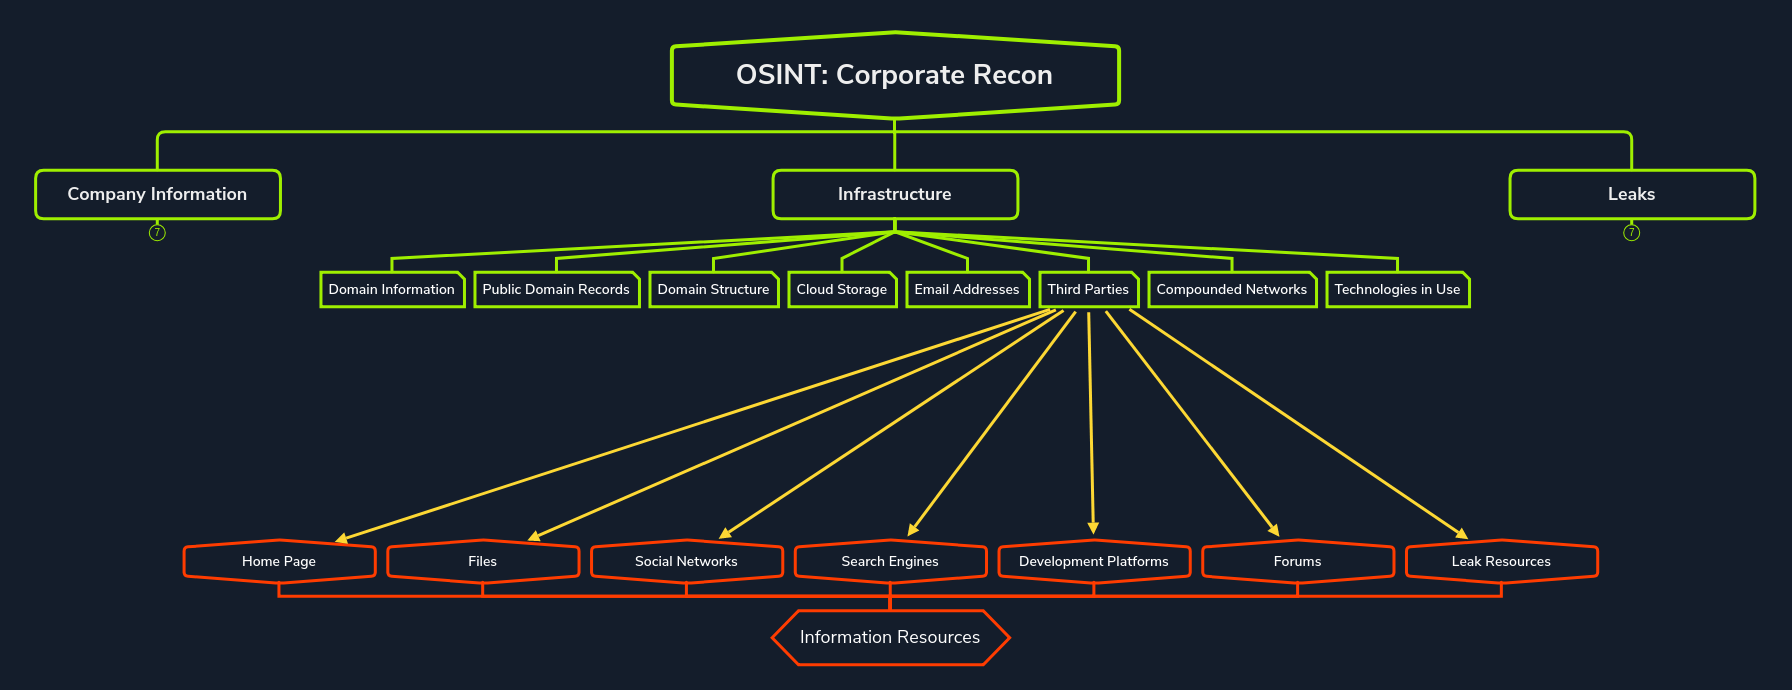
\includegraphics[width=\linewidth]{recon/osint/images/infra-3rd-parties.png}
  \caption{OSINT Infra third parties}
  \label{fig:osint-infra-3rd-parties}
\end{figure}

We can see from the graph that we can get this information about third-party
vendors from pretty much any information resource. We will go through the
information resources that we have transferred to our Resource Browser in this
step. If we have followed the methodology, we already have many information
resources such as different websites, providers, files, and images that we can
use for this. Here we need to summarize them and get an overview of how the
company is positioned and which providers are used.

Apart from the different software the company uses, the hosting providers play
an essential role. Based on this, we will assess how extensive the inventory is
in the cloud, if at all, and what these {\bf hosting providers} offer for
security measures.


\subsubsection{Hosting Provider}

It is always necessary to establish who the third-party providers are and what
services they provide to the company. This should always be discussed in the
meetings before the penetration test.

\href{https://securitytrails.com/}{SecurityTrails} does an excellent job in
this research, which we should take advantage of.

Based on these results, we determined the four different hosting providers that
our target company uses. We can search for the names of the hosting providers
on Google, for example, and see their penetration test policies and rules of
engagement and how best to get permissions for them.

If we do not find a hosting provider in the list, it is most likely a
self-hosted system.

\subsubsection{Documents}

Here we should take a closer look at the providers who could make files
available to us. These files can contain valuable information about the company
itself and its processes and show us whom they work with to manage the
infrastructure. For this search, we use the search engines like Google with the
dork \verb+site:+ which will limit our searches to the pages we need. The most
used providers for documents include, but are not limited to:

\begin{verbatim}
Google Docs 	        site:docs.google.com
Google Cloud 	        site:cloud.google.com
Google Storage 	        site:storage.googleapis.com
Microsoft 	            site:docs.microsoft.com
Amazon Web Services 	site:amazonaws.com
\end{verbatim}


\subsection{Compounded Networks}

Compounded networks use platforms that are suitable for both {\bf personal} and
{\bf business} purposes. The difference between information sharing and
information dissemination is that people on these platforms disclose less
information about themselves. They want to make sure that potential employers
or their current employers do not get the wrong impression. Confrontation is an
essential aspect of professional life that every employee wants to avoid.

\begin{figure}
  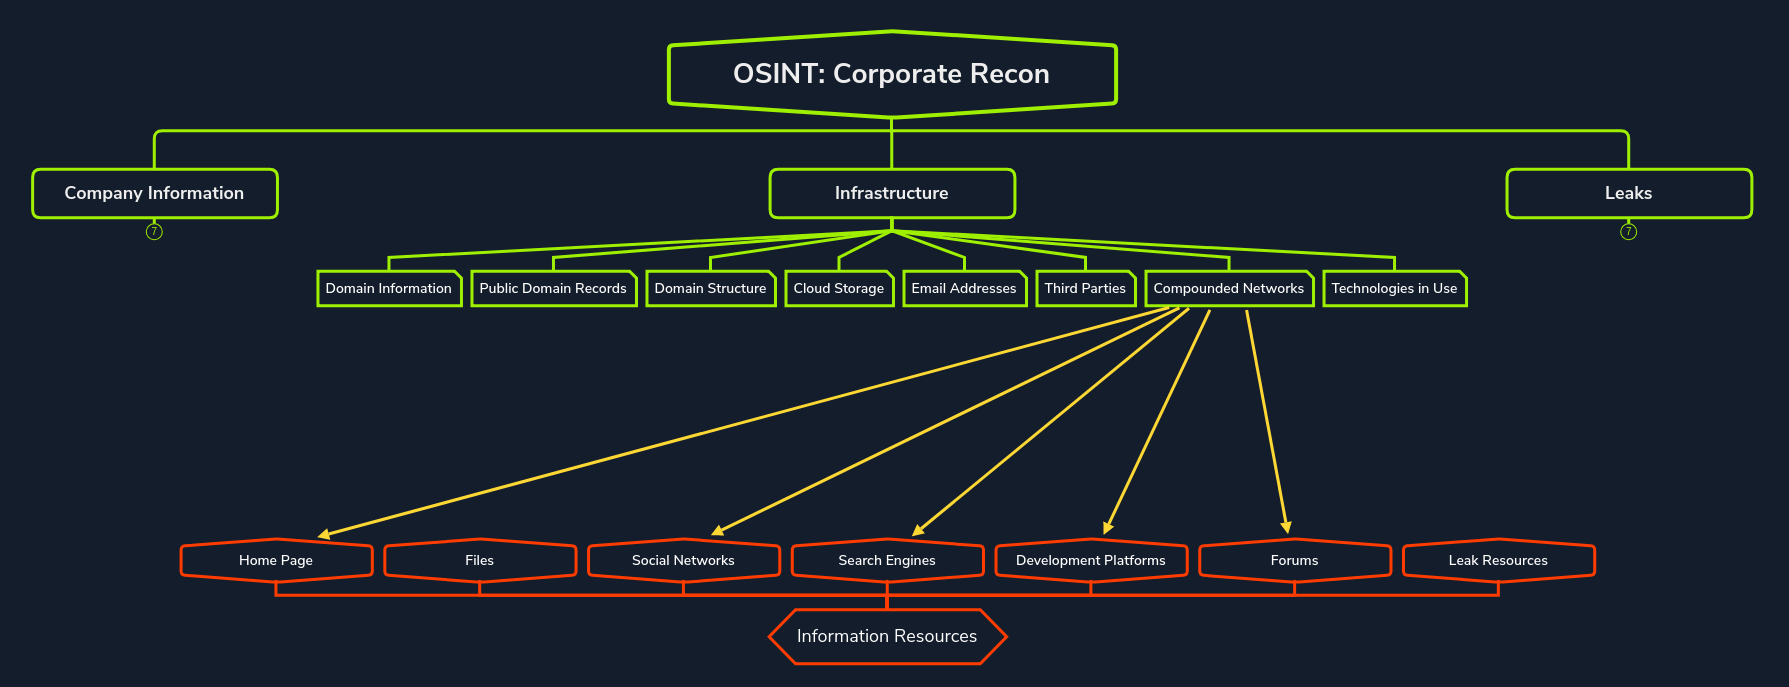
\includegraphics[width=\linewidth]{recon/osint/images/infra-networks.png}
  \caption{OSINT Infra Compounded Networks}
  \label{fig:osint-infra-networks}
\end{figure}
In most cases, we can already find all the links to the social networks on
which the company is linked on the company's home page. The best known
compounded social media platforms are, but not limited to: Facebook, Instagram,
Twitter

Another essential difference between real conversations and opinions on social
media platforms is that people often express views on a topic that they would
not usually have the courage to communicate in a face-to-face conversation.
This is because people feel safe to express their opinions at a distance
without the risk of provoking direct conflict, and above all, they have much
more time to respond than in a face-to-face conversation.

By reading through such comments and posts, we can create a pattern of how our
target employee thinks about a specific topic. Above all, security-relevant
information may be published when one is actually looking for help. However,
the stress and worry that we get careless and unfocused can lead to such
publications of security-related information.

Furthermore, posts on these platforms can also draw attention to illegal
activities by the employee. Suppose our employee, as an example, has taken
specific courses and training paid for by our client, and the employee shares
this publicly with all others. In that case, it is a violation of the general
terms and conditions for which our client is liable and accordingly also
security-relevant. We cannot say whether company-specific information has been
shared, but we should investigate the employee more in detail to prove or
disprove this fact.

\subsubsection{Social Networks}

Here we focus not on the search for compounded social networks but the content
within them. For this purpose, the corresponding {\bf hashtags} are suitable,
which primarily connect users with the company. In addition to the individual
persons, partners can also be recognized, since they often thank them for a
friendly comment or can also make themselves known through some other
activity.

The focus here is on finding social groups created either by the company
itself, its employees, or third parties in which specific topics are discussed.
In doing so, we should narrow down the search for these groups as best we can
with the information we have already obtained. After all, if we search only for
Java, we will get quite a few results that will make our work more difficult.
However, if we use several terms, such as \verb+Java + target-company + web
interface+, we will reduce our search results many times and become much more
precise.

Basically, in compounded social networks, we can obtain internal information
that is not directly visible. To do this, we should examine fields such as
groups, comments, images, and the like. It is crucial to trace the entire
conversation as best as possible and try to find out the background and why and
how it came about that this conversation is taking place. Complaints that
reflect employees' internal impressions of the company are excellent indicators
of this.

\subsection{Technologies in Use}

One of the most valuable pieces of information about the infrastructure is the
technologies the company uses. Often it is not always easy to get much of this
information passively. However, we do have some tools at our disposal to help
us extract this information. Here, too, any information resource can be of
great importance. The focus here is on identifying technologies that we can
later use to adapt our attacks against the company. Especially for social
engineering attacks, this plays an important role later on. We can interact
with the employees and communicate and build trust with customized information
(which only trusted people know).

\begin{figure}
  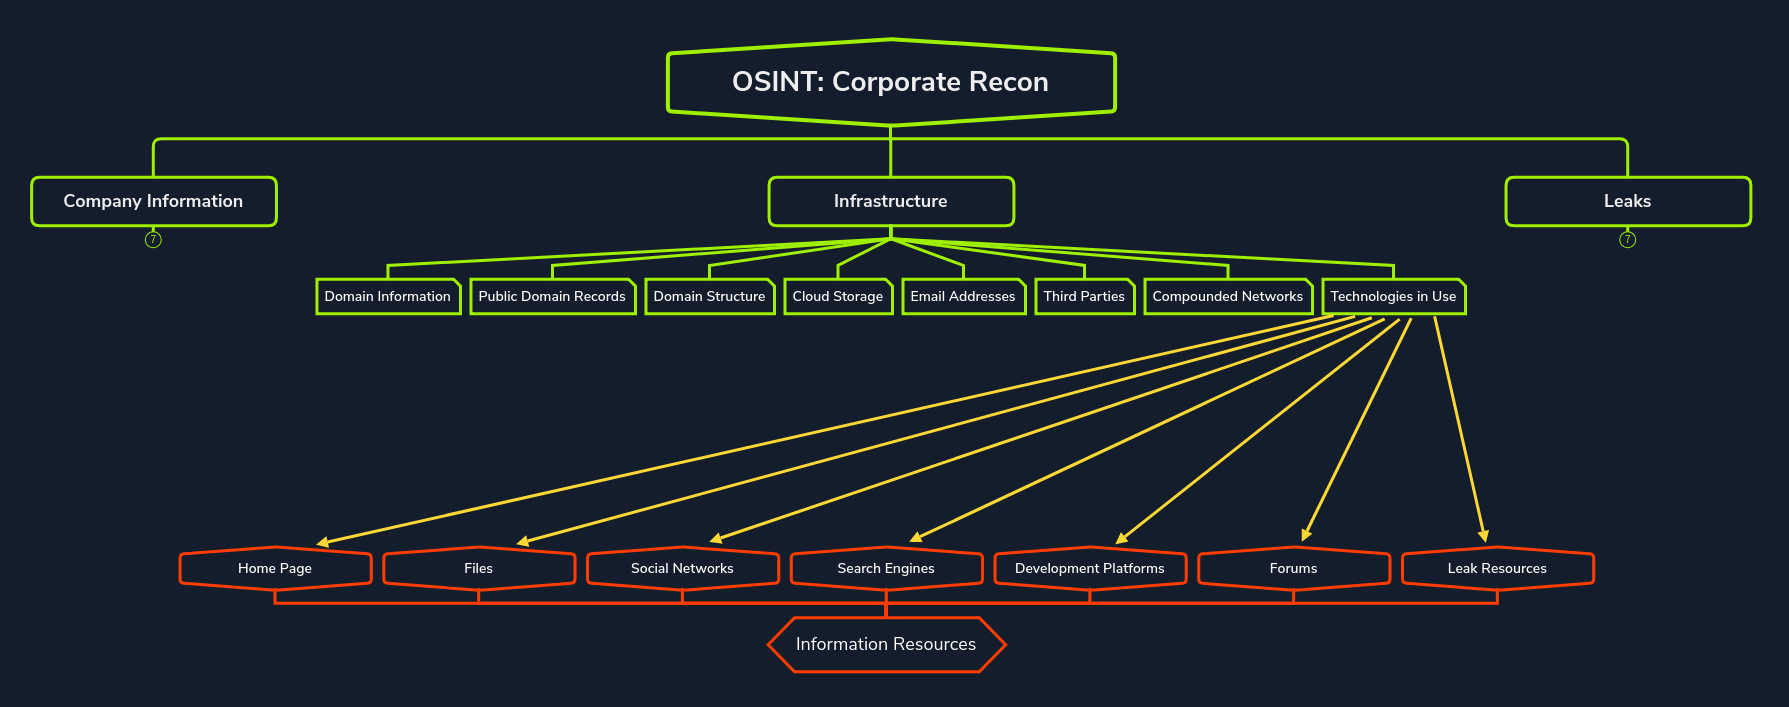
\includegraphics[width=\linewidth]{recon/osint/images/infra-techs.png}
  \caption{OSINT Infra Technologies}
  \label{fig:osint-infra-techs}
\end{figure}
Such information includes any software or provider that makes such an
application available. Once we understand what the company is using
technologies, this will give us a reasonably accurate picture of the aspects
that will be most relevant to us as we prepare our attack on the company.


\subsubsection{Home Page}

We can already learn a lot of information from a company's home page. This can
be, for example, different forms or content from the source code of the page.
Especially with CMS, like WordPress applications, it is quite helpful because
they are individually combined with different plugins. Often, weak points are
found in the individual plugins, which can then be exploited to penetrate the
company's network.

Another beneficial source that can tell us a lot about the target company's
website alone is \href{https://builtwith.com/}{BuiltWith}. It lists all the
technologies that are used by the web server and are deployed on it.

BuiltWith analyzes the content of the website and identifies the technologies
used for it. This gives us an even better overview of how the web developers
work and their knowledge, which we can use to assess how experienced they are.
This is because we can use our assessments to identify or rule out certain
security-related aspects, making our attack vector much more straightforward.

\subsubsection{Search Engines}

In the section Public Domain Records, we already used the Shodan CLI to find
information about the respective IP addresses. Shodan showed us which services
it recognized and the technologies behind them. We can get the necessary
information about the domain from Shodan using the "domain" parameter and see
what details we will find about it. Most of the time, we get a good insight
into the systems related to the domain, and sometimes we can even identify the
vhosts directly, apart from the subdomains. Sometimes we can even find other
domains with different TLDs that extend our attack vector if the scope in the
contract allows it.
\begin{verbatim}
shodan domain target-company.com
\end{verbatim}

hodan also has databases in which information is stored over a specific and
relatively long period. We can use the Shodan CLI to search this database for
entries related to our target company.

\begin{verbatim}
shodan search target-company | cut -d" " -f1-3
\end{verbatim}
